\documentclass[a4paper, 12pt, english]{article}
\usepackage[utf8]{inputenc}
\usepackage{fancyhdr}
\usepackage{graphicx}
\usepackage{lastpage}
\usepackage{layout}
\usepackage{enumitem}
\usepackage{etoolbox}
\usepackage{amsmath}
\usepackage{mathptmx}
\usepackage[bottom]{footmisc}
\usepackage[includeheadfoot, left=3cm, right=3cm, top = 1.5 cm]{geometry}
\usepackage{minted}
\usemintedstyle{xcode}


\graphicspath{ {./answers/} }

\pagestyle{fancy}
\fancyhf{} 
\rhead{
    {\Large \textbf{Analysis and Design of Algorithms}}\\
    \textbf{CS2102} \\ 
    \textbf{Divide and Conquer Practice} \\ 
    \textbf{2020-II}
}
\lhead{
\includegraphics[width=4.6cm, keepaspectratio]{logo/utec}}
\rfoot{\textbf{\thepage}\hspace{1pt} of \textbf{\pageref{LastPage}}}
\cfoot{}

\setlength{\parindent}{0em}
\setlength{\headheight}{80pt}

\newcounter{problem}[section]
\newenvironment{problem}[3][]{\refstepcounter{problem}\par\medskip 

\textbf{Problem~\theproblem  ~~(#2) - 
\ifboolexpr{
  test {\ifdimless{1 pt}{#3 pt}}
}
{#3 points} % true
{#3 point} % false
} \newline\newline } {\medskip} 


\begin{document}

\textbf{Submission deadline}: 23 December, 08:10

\begin{itemize}
    \item Write your answers (images) inside the \emph{answers} folder in order to generate a single PDF file. Replace the image files that are already included in the project. Do not change the file name.
    \item Read the questions carefully and write your answers clearly. Answers that are not legible and that doesn't follow the format will not have any score. 
\end{itemize}

\underline{Outcomes}:

\begin{enumerate}[label=\alph*.]
    \item Apply appropriate mathematical and related knowledge to computer science.
    \item Analyze problems and identify the appropriate computational requirements for its solution.
\end{enumerate}
\noindent\rule{\textwidth}{0.01pt}
\vspace{3mm}

\begin{problem}{Outcome b}{3}
    Explain what is an NP-complete problem and how can you determine that a problem is NP-complete in terms of reductions? Define the Independent Set and Vertex Cover problems and explain the reduction between them.
    
    \begin{center}
        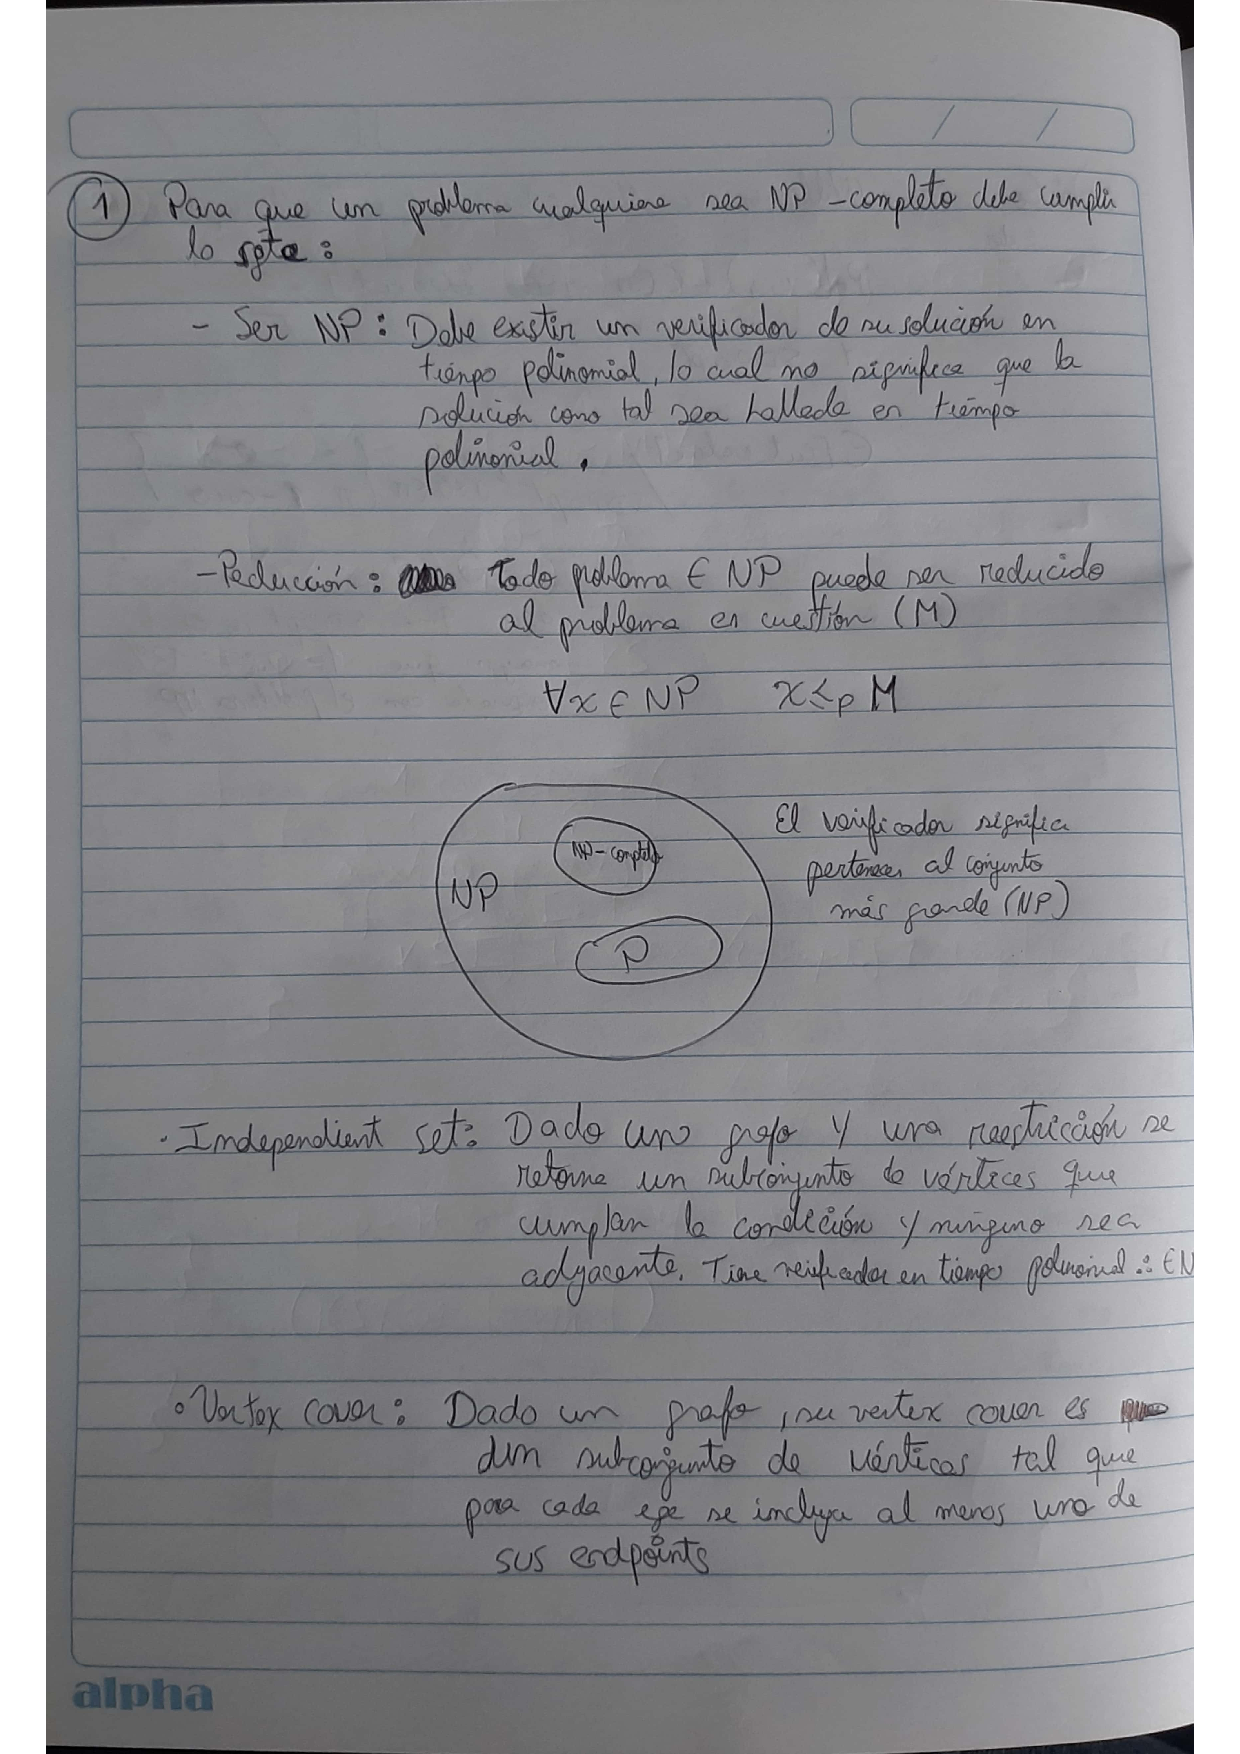
\includegraphics[width=0.9\linewidth]{problem1/problem1}%
    \end{center}

\end{problem}

\begin{problem}{Outcomes a, b}{5}

\begin{itemize}
        \item Consider the 0-1 knapsack problem variation to write the recurrence relation and the pseudocode of an algorithm using Dynamic Programming. The algorithm should receive the $n$ items (with its respective weights and values) and a maximum capacity $M$ and return the maximum value supported by the bag. Your algorithm should have a complexity of O(n*M) and be restricted to a space consumption of O(M).
        
        \item Based on the algorithm written above construct the dynamic programming table using the following information assuming that $M=15$. 
        
        \begin{center}
            \begin{tabular}{S|SSSSSSS} \toprule
                \text{Item}          & 1 & 2 & 3 & 4 & 5 & 6 & 7  \\ \midrule
                \text{Weight (kg)}   & 3 & 8 & 6 & 2 & 1 & 9 & 10 \\
                \text{Value (\$)}    & 1 & 7 & 8 & 4 & 2 & 5 & 3  \\ \bottomrule
            \end{tabular}
        \end{center}
    \end{itemize}
\begin{center}
    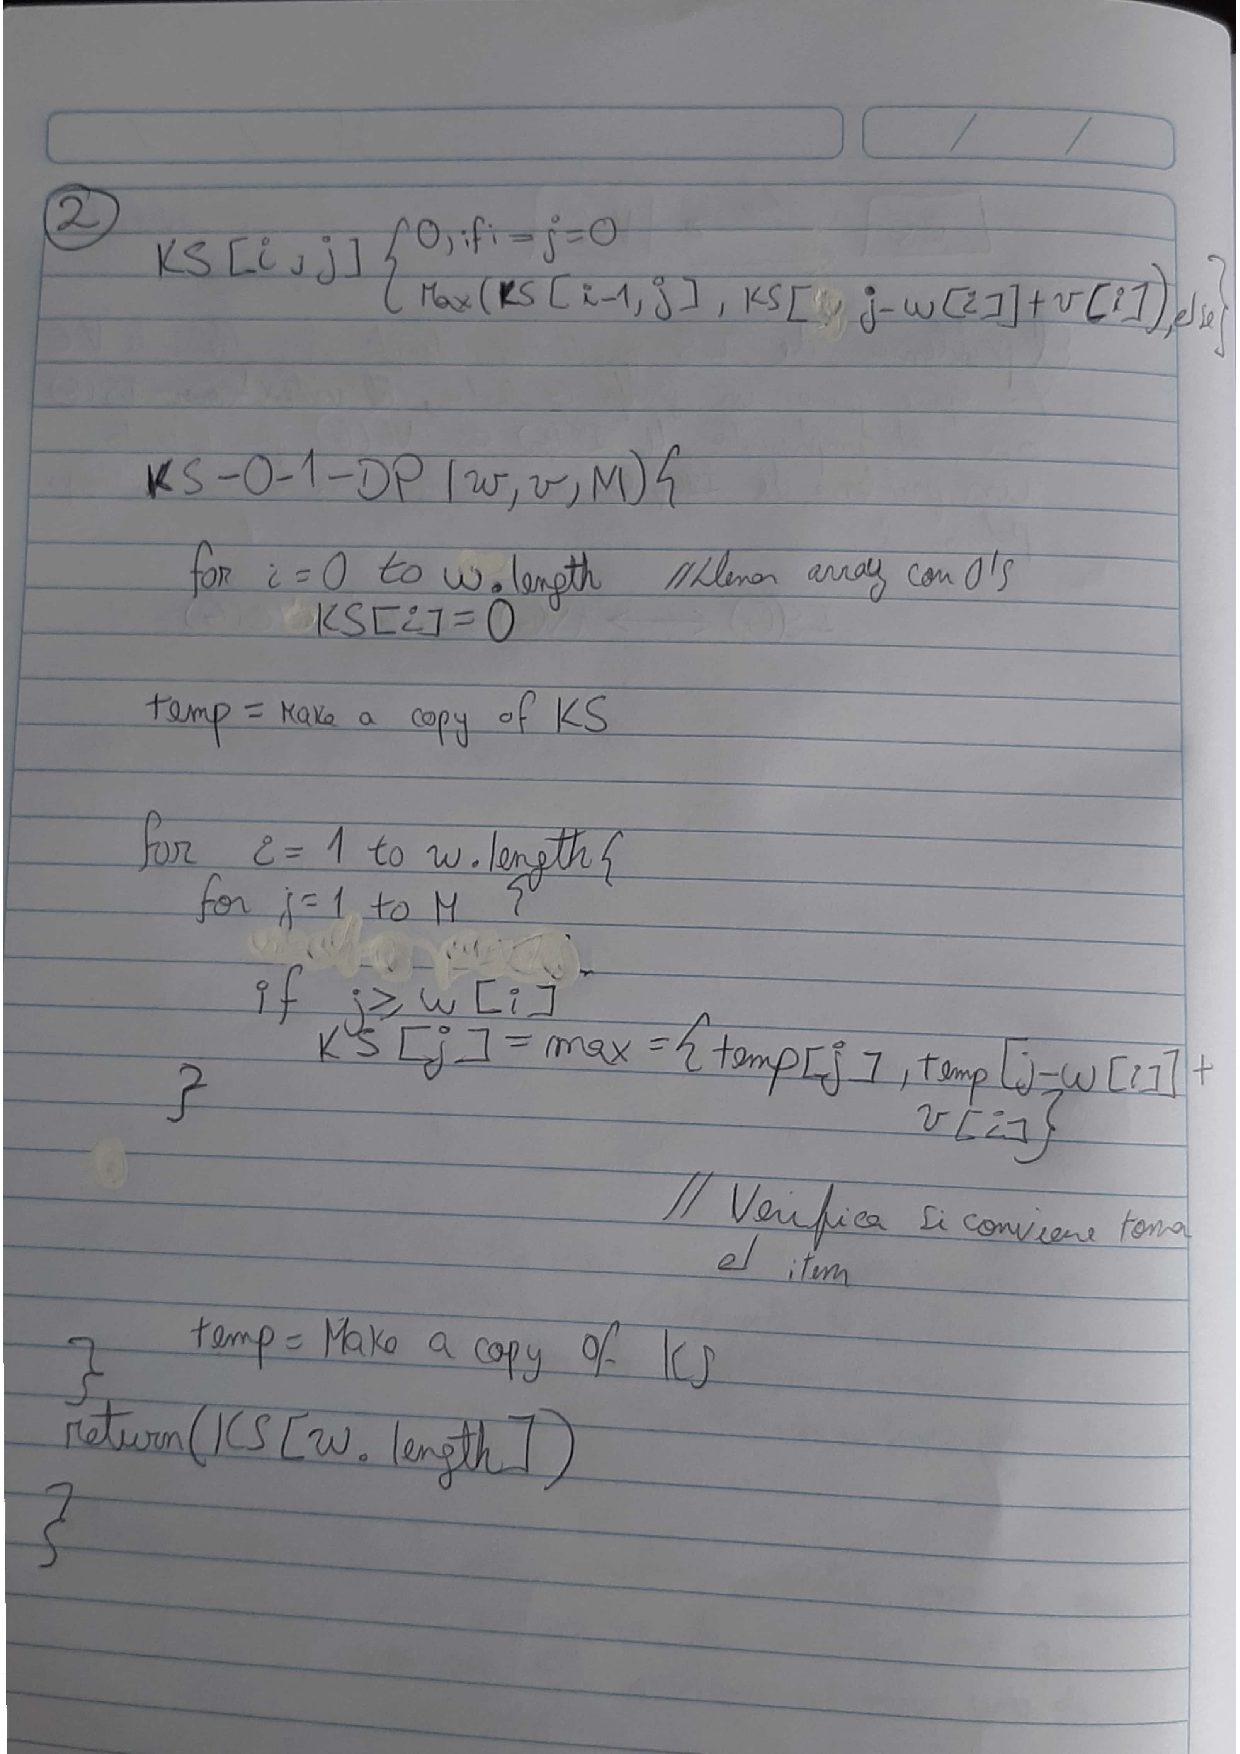
\includegraphics[width=0.9\linewidth]{problem2/problem2}%
\end{center}

\end{problem}

\begin{problem}{Outcomes a, b}{4}
Given a rod of $n$ meters and an array that contains prices of all pieces of size smaller than $n$:
\begin{itemize}
    \item Write the recurrence relation and the pseudocode of an algorithm using dynamic programming to find the optimal way to cut the rod into smaller rods in order to maximize the profit.
    \item Consider the information below and construct the dynamic programming table to find the optimal way to cut the rod and maximize profit. Write your answer clearly.
    \begin{center}
        \begin{tabular}{S|SSSSS}
            \text{Length ($i$)}  & 1 & 2 & 3 & 4 & 5 \\ \midrule
            \text{Price ($p_i$)} & 1 & 5 & 8 & 9 & 10 \\
        \end{tabular}
    \end{center}
\end{itemize}

\begin{center}
    
\includegraphics[width=0.9\linewidth]{problem3/problem3}%
\end{center}

\end{problem}

\begin{problem}{Outcome b}{4}
    Choose one of the topics presented during the Final Project presentations and write a brief and concise definition of the problem, applications, foundation and analysis of your selected algorithm.

    \begin{center}
        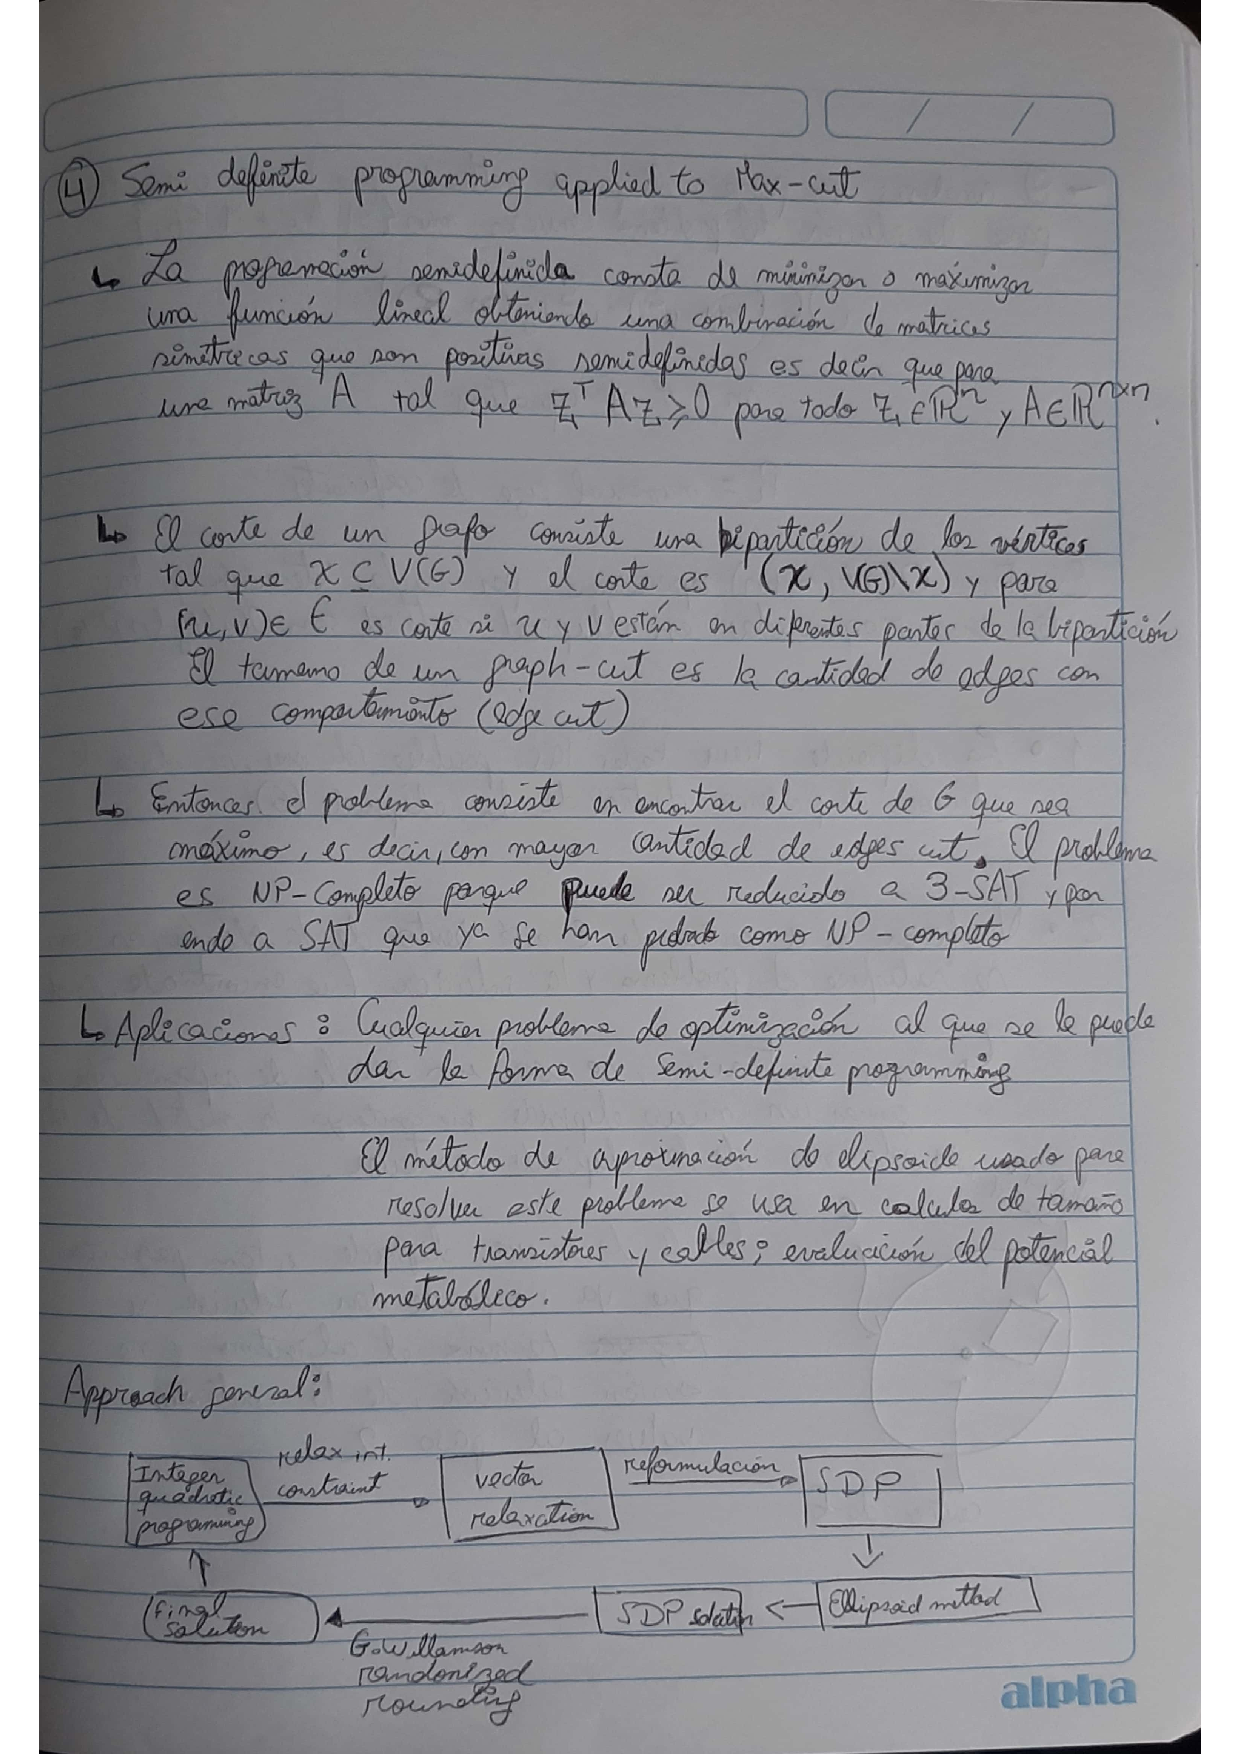
\includegraphics[width=0.9\linewidth]{problem4/problem4}%
    \end{center}

\end{problem}

\begin{problem}{Outcome b}{4}
A company produces two products: A and B. 
The production of each product of type A requires 3 hours to build and 1 hour to wrap up.
The production of each product of type B requires 4 hours to build and 3 hours to wrap up. 
For building and wrapping up a product the maximum available hours are 60 and 30 respectively. 
The company makes a profit of \$8.000 on each item of product A and \$12.000 of each item of product B. 
How many items of product A and B should be produced to maximize the profit ? What is the maximum profit? Assume non-negative constraints and plot the inequalities highlighting the feasible region.\newline

Remarks: Write all the operations of the row reduction process.

\begin{center}
    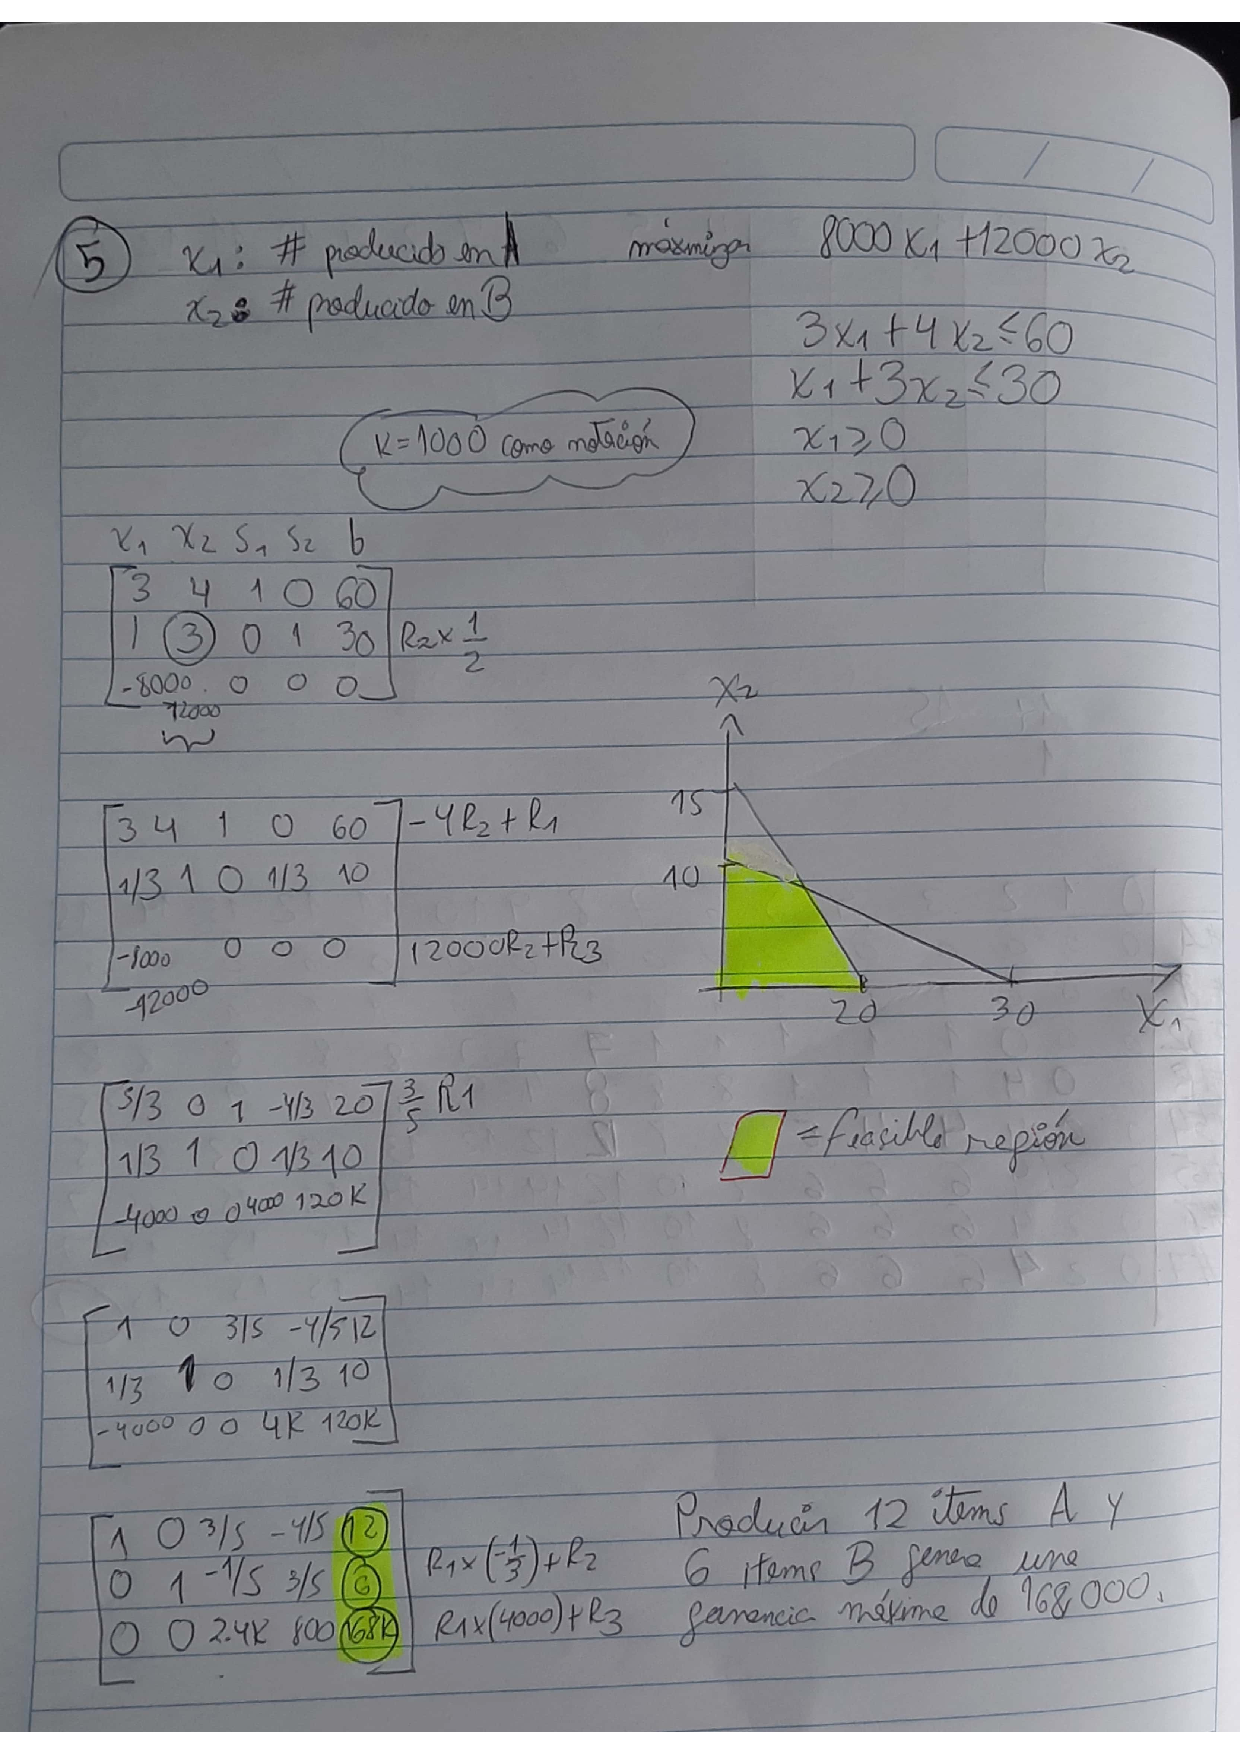
\includegraphics[width=0.9\linewidth]{problem5/problem5}
\end{center}

\end{problem}

\end{document}



